\section{Multilingual Topic Model for Connecting Cross-Lingual Topics}
%\section{Model}
\label{sec:model}


%\begin{figure}[t!]
%  \centering
%  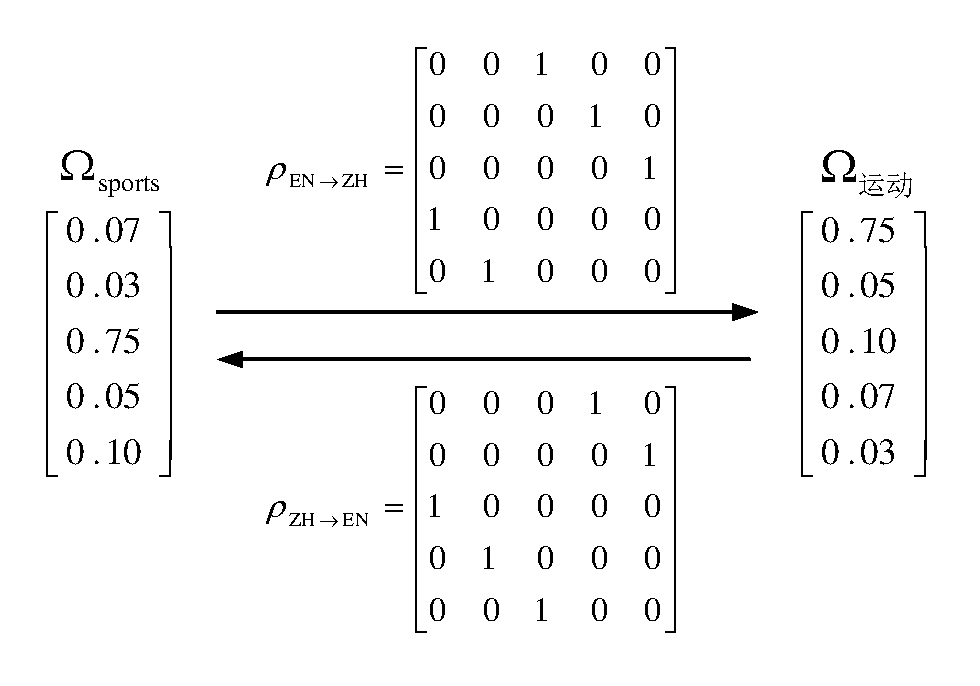
\includegraphics[width=.935\linewidth]{2019_emnlp_mtm/figures/rho.pdf}
%  \caption{Our model uses topic link weight matrices~$\bm{\rho}$'s to
%    transform topics from one language to another.  Unlike other
%    models, it allows a topic to linked to another topic or multiple topics.}
%
%  \label{fig:rho}
%\end{figure}

\newcite{yang-2015-knowledge} present a flexible framework for adding
regularization to topic models.  We extend this model to the
multilingual setting by adding a potential function that links topics
across languages.  For simplicity of exposition, we focus on the
bilingual case with languages~$S$ and~$T$.


\jbgcomment{I think this contrast could be a little clearer.  All of the models there are monolingual, etc.  It's not just that there are two matrices\dots \wycomment{Is it better now?}}

Unlike~\newcite{yang-2015-knowledge} that encode monolingual information only, our potential function encodes multilingual knowledge parameterized
by two matrices,~\rhost and~\rhots, that transform topics between the two languages.
Cells' values are between 0 and 1 and a cell $\rho_{S \rightarrow T, k_T, k_S}$ close to one is a strong connection of topics~$k_T$ and~$k_S$ in language~$T$ and~$S$.  \jbgcomment{``while transforming'' is vague; make clearer. \wycomment{Looks like it is clearer if not mentioning transformation.}}
Transformations~$\bm{\rho}$ are learned from translation pairs' topic
distributions.

These topic distributions come from the assignments of Gibbs
sampling~\cite{griffiths-2004-lda-gibbs}.
%
Fortunately adding the potential function is equivalent to adding an
additional term to Gibbs sampling for topic
models~\cite{yang-2015-knowledge}.
%
During sampling, each token is assigned
to a topic, so we can compute a \emph{post
  hoc} word distribution over topics. The probability of a topic~$k$ given a word~$w$ is $\prob{k}{w} \equiv \Omega_{w,k}
\equiv N_{k,w} / N_w$, where~$N_{k,w}$ is the number of times that
word~$w$ is assigned to topic~$k$ and~$N_w$ is~$w$'s term frequency.

\jbgcomment{Expand this out a little bit; explicitly say that this is
  the probability of topic given a word. \wycomment{Done.}}

To find good topic links~\rhost, we use a dictionary.
%
For instance, given the translation pair of ``sports'' and ``\ch{运动}
(\pinyin{yun4} \pinyin{dong4})'', they should have similar topic distributions, so we want $\bm{\rho_{\text{\en}
    \rightarrow \text{\zh}}} \bm{\Omega_{\text{sports}}}$ to be
close to $\bm{\Omega_{\text{\ch{运动}}}}$ and vice versa. \jbgcomment{Make this clearer: these words should have similar topics.\wycomment{Done.}}
%
Moreover, the transformations should be symmetric:  $\bm{\rho_{S
    \rightarrow T}} \bm{\Omega_{w_S}}$ close to~$\bm{\Omega_{w_T}}$,
and vice versa. \jbgcomment{Explaing what ``consistent'' means with words: one transform should be the inverse of the other.\wycomment{Maybe ``symmetric'' is a better word here?}}
We encode this cross-lingual
knowledge of topic transformations into the potential function~$\Psi$ which measures the difference of translation pairs' topic distributions after transformation\ignore{as the reciprocal product
of all translation pairs' topic distribution distances after
transformation by~$\bm{\rho}$}:  \jbgcomment{Explain with words what this equation is trying to do; don't just say ``close to''.\wycomment{Done.}}
\begin{equation}
\small
\left( \prod_{c=1}^{C} \left\lVert \bm{\Omega_{S,c}} - \bm{\rho_{T \rightarrow S}} \bm{\Omega_{T,c}} \right\rVert_{2}^{\eta_c} \left\lVert \bm{\rho_{S \rightarrow T}} \bm{\Omega_{S,c}} - \bm{\Omega_{T,c}} \right\rVert_{2}^{\eta_c} \right)^{-1}, \label{equ:psi}
\end{equation}
where~$\eta_c$ is the statistical importance of the~$c$-th translation pair to the corpus \jbgcomment{``importance'' is vague, rename or be more specific. \wycomment{Elaborated a little bit. Is it better?}}
(Figure~\ref{fig:mtm_model}, full
details in the Supplement).
\begin{figure}[t]
  \centering
  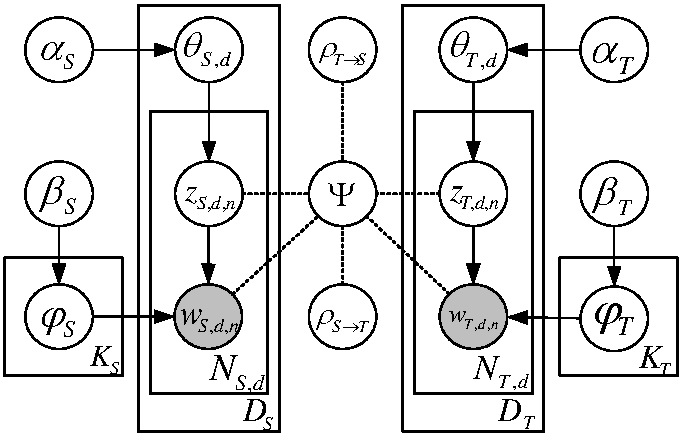
\includegraphics[width=\linewidth]{2019_emnlp_mtm/figures/mtm2.pdf}
  \caption{The graphical model of our multilingual topic model. The
    topic links~$\bm{\rho}$, as instantiated by the function $\Psi$,
    encourage topics to encourage word translations to have
    consistent topics.}
\label{fig:mtm_model}
\end{figure}

\ignore{
:\par\nobreak
\begin{small}
\begin{enumerate}[leftmargin=*,noitemsep]
  \item For each topic $k \in \{ 1, \ldots, K_T \}$ in language~$T$
  \begin{enumerate}
    \item Draw word distribution $\bm{\phi_{T,k}} \sim \text{Dir} (\beta_T)$.
  \end{enumerate}
  \item For each document $d \in \{ 1, \ldots, D_T \}$ in language~$T$
  \begin{enumerate}
    \item Draw topic distribution $\bm{\theta_{T, d}} \sim \text{Dir} (\alpha_T)$.
    \item For each token $t_{T,d,n}$ in document~$d$
    \begin{enumerate}
      \item Draw a topic $z_{T,d,n} \sim \text{Mult} (\bm{\theta_{T,d}})$.
      \item Draw a word $w_{T,d,n} \sim \text{Mult} (\bm{\phi_{T,z_{T,d,n}}})$.
    \end{enumerate}
  \end{enumerate}
  \item For each topic $k \in \{ 1, \ldots, K_S \}$ in language~$S$
  \begin{enumerate}
    \item Draw word distribution $\bm{\phi_{S,k}} \sim \text{Dir} (\beta_S)$.
  \end{enumerate}
  \item For each document $d \in \{ 1, \ldots, D_S \}$ in language~$S$
  \begin{enumerate}
    \item Draw topic distribution $\bm{\theta_{S,d}} \sim \text{Dir} (\alpha_S)$.
    \item For each token $t_{S,d,n}$ in document $d$
    \begin{enumerate}
      \item Draw a topic $z_{S,d,n} \sim \text{Mult} (\bm{\theta_{S,d}})$.
      \item Draw a word $w_{S,d,n} \sim \text{Mult} (\bm{\phi_{S,z_{S,d,n}}})$.
    \end{enumerate}
  \end{enumerate}
  \item Draw the posterior regularizer~$\Psi$ with Equation~\ref{equ:psi}.
\end{enumerate}
\end{small}
}

\jbgcomment{Make it clearer that the models there don't have additional parameters, but we do (and say what those parameters are).\wycomment{Done.}}
While~\newcite{yang-2015-knowledge} provide a blueprint for Gibbs
sampling with potential functions without additional parameters,
our model has additional parameters of~\rhost and~\rhots so we need to optimize them.
Thus, we use stochastic
\textsc{em}~\cite{celeux-1985-sem}. The E-step updates tokens'
topic assignments using Gibbs sampling, while holding the parameters of the
topic link weight matrices~$\bm{\rho}$ fixed.
%\footnote{The equations in E-step and the optimization
%  for~\rhots in M-step are available in Supplement.}
The M-step optimizes~$\bm{\rho}$ while holding the topic
assignments fixed. We\jbgcomment{I would instead say that you optimize in log space\wycomment{Done.}}
optimize~$\Psi$ in log space using the objective
function~$J(\bm{\rho_{S \rightarrow T}})$ as
\begin{equation}\label{equ:rho_obj}
\small
\sum_{c=1}^{C} \eta_c \log \left\lVert \bm{\Omega_{T,c}} - \bm{\rho_{S \rightarrow T, i_T}} \bm{\Omega_{S,c}} \right\rVert_{2},
\end{equation}
which is minimized by using \lbfgs~\cite{liu-1989-lbfgs}, with the
partial derivatives with respect to~$\rho_{S \rightarrow T, k_T, k_S}$
\begin{equation}\label{equ:rho_grad}
\small
- \sum_{c=1}^{C} \frac {\eta_c \Omega_{S,c,k_S} \left( \Omega_{T,c,k_T} - \bm{\rho_{S \rightarrow T, k_T}} \bm{\Omega_{S,c}} \right)} {\left\lVert \bm{\Omega_{T,c}} - \bm{\rho_{S \rightarrow T, i_T}} \bm{\Omega_{S,c}} \right\rVert_{2}^2}.
\end{equation}
